\pdfoutput=1
\pdfminorversion=4

\documentclass[preprint]{elsarticle}
\usepackage[utf8]{inputenc}

%packages
\usepackage[margin=1in]{geometry}

\usepackage[hyphens]{url}
\biboptions{sort&compress, square, comma}
\usepackage[breaklinks=true, linkcolor=blue, citecolor=blue, colorlinks=true]{hyperref}

\usepackage{graphicx}
\usepackage{caption}
\usepackage{subcaption}

\usepackage{booktabs}

\usepackage[version=3]{mhchem} % Formula subscripts using \ce{}, e.g., \ce{H2SO4}
\usepackage{latexsym,amsmath,amssymb}

\usepackage{mathtools}
\usepackage{tablefootnote}

%better printing of numbers
\usepackage[T1]{fontenc}
\usepackage[english]{babel}
\usepackage{csquotes}
\usepackage{textcomp}

\usepackage{algorithm}
\usepackage[noend]{algpseudocode}
\makeatletter
\let\OldStatex\Statex
\renewcommand{\Statex}[1][3]{%
  \setlength\@tempdima{\algorithmicindent}%
  \OldStatex\hskip\dimexpr#1\@tempdima\relax}

\usepackage[binary-units]{siunitx}
\sisetup{group-separator={,},
     detect-all,
     binary-units,
     list-units = single,
     range-units = single,
     tophrase = --, 
     per-mode = symbol-or-fraction,
     separate-uncertainty = true,
     list-final-separator = {, and }
%    scientific-notation = fixed
}
\DeclareSIUnit\atm{atm}

% Add [disable] option to quickly remove any
\usepackage[textsize=small,textwidth=2.5cm]{todonotes}

%custom commands
\newcommand{\NA}{---}
\newcommand{\centercell}[1]{\multicolumn{1}{c}{#1}}
\newcommand{\centermulti}[2]{\multicolumn{#2}{c}{#1}}
\newcommand{\head}[1]{\centercell{\bfseries#1}}
\newcommand{\headmulti}[2]{\centermulti{\bfseries#1}{#2}}

\journal{36th International Symposium on Combustion}

\begin{document}
\begin{frontmatter}

\title{An Investigation into GPU accelerated Chemical Kinetic Integration}

\author[uconn]{Nicholas~J.\ Curtis}
\author[osu]{Kyle~E.\ Niemeyer}
\author[uconn]{Chih-Jen Sung\corref{cor1}}
\ead{cjsung@engr.uconn.edu}

% addresses
\address[uconn]{Department of Mechanical Engineering\\
  University of Connecticut, Storrs, CT, 06269, USA}
\address[osu]{School of Mechanical, Industrial, and Manufacturing Engineering\\
  Oregon State University, Corvallis, OR 97331, USA}
  
\cortext[cor1]{Corresponding author}

\begin{abstract}
TODO
\end{abstract}

\begin{keyword}
 Chemical kinetics \sep Stiff chemistry \sep SIMD \sep GPU
\end{keyword}

\end{frontmatter}

%%%%%%%%%%%%%%%%%%%%%%%%%%%%%%%%%%%%%%%%%%%%
\section{Introduction}
\label{sec:Intro}
%%%%%%%%%%%%%%%%%%%%%%%%%%%%%%%%%%%%%%%%%%%%

The need for accurate chemical kinetic models in predictive reacting-flow simulations has driven the development of detailed oxidation models for hydrocarbon fuels relevant to transportation and energy generation applications.
At the same time, growing understanding of the hydrocarbon oxidation process resulted in orders of magnitude increases in model size and complexity.
For instance, a recently developed model for 2-methylalkanes, relevant for jet and diesel fuel surrogates, consists of over 7000 species and 30000 reactions~\cite{Sarathy:2011kx} while a recent detailed gasoline surrogate mechanism contains over 1500 species and 6000 reactions~\cite{Mehl:2011jn}.
Furthermore, kinetic models for large hydrocarbon fuels tend to exhibit chemical stiffness requiring implicit integration algorithms~\cite{Lu:2009gh}, the solution cost of which scale at best quadratically---and at worst cubically---with the number of species in a mechanism~\cite{Lu:2009gh}.

Consequently, a number of techniques have been developed to accelerate chemical kinetics integration.
As Lu and Law reviewed more extensively~\cite{Lu:2009gh}, these methods can be roughly categorized into three classes: skeletal reduction and removal of unimportant species and reactions~\cite{Lu:2005,Pepiot-Desjardins:2008,Niemeyer:2010bt,Niemeyer:2014,Curtis:2015aa}, time-scale analysis~\cite{qssa,pe_approx1,pe_approx2} and dimensional reduction~\cite{Lam:1988wc,Maas:1992aa,Lu:2001ve}, and tabulation\slash interpolation of expensive terms~\cite{Pope:1997wu,Christo1996}.
In addition to these cost-reduction methods, significant work has been directed towards improvements of the integration algorithms themselves.

Reacting-flow modeling codes typically rely on high-order implicit integration techniques to efficiently solve the stiff governing equations typically exhibited by chemical kinetics models.
These methods require repeated evaluation and factorization of the chemical kinetic Jacobian matrix in order to solve the associated non-linear algebraic equations through iterations of linear system solutions, the cost of which scales quadratically and cubically, respectively, with the number of species in a mechanism.
However, significant cost savings in the Jacobian evaluation can be realized through the use of an analytic formulation, rather than the typical evaluation via finite difference approximations.
This approach eliminates numerous chemical source term evaluations, and the cost of Jacobian evaluation drops to a linear dependence on the number of species in the mechanism~\cite{Lu:2009gh}.
Several analytical Jacobian matrix codes have been developed~\cite{Safta:2011vn,Youssefi:2011tm,Bisetti:2012jw,Perini:2012gy,Dijkmans:2014bb}, but the recently released \texttt{pyJac} software~\cite{Niemeyer:2015im,Niemeyer:2015ws} is currently the only open-source analytical chemical kinetic Jacobian tool capable of both generating code for new SIMD processor types, as well as handling newer pressure dependence formulations (e.g., pressure-log or Chebyshev rate formulations).

Further acceleration of chemical kinetic integration techniques has focused on improvements to the integration itself, via development of new algorithms and use of high-performance hardware accelerators such as as graphics processing unit (GPUs) and other similar single-instruction multiple-data (SIMD) devices.
Central processing unit (CPU) clock speeds increased regularly over the past few decades---commonly known as Moore's Law---however, power consumption and heat dissipation have issues slowed this trend recently.
While multi-core parallelism somewhat increased CPU performance, recently SIMD processors have gain popularity as a low cost, low power consumption, and massively parallel high-performance computing alternative.
GPUs were originally developed for graphics\slash video processing applications and consist of hundreds to thousands of separate cores, compared to the tens of cores found on typical CPUs.
The SIMD parallelism model is very different from a traditional CPU based multi-threading model, with small per-core memory caches and accelerations resulting from executing the same instruction on multiple data sets.
For more details, the reader is referred to several works which have discussed these differences in depth~\cite{Cruz:2011gc,Brodtkorb:2013hn,Niemeyer:2014hn}.

A number of studies in recent years explored the use high-performance SIMD devices for acceleration of turbulent reacting flow simulations.
Spafford et al.~\cite{Spafford:2010aa} first investigated the use of GPUs to accelerate a turbulent combustion direct numerical simulation code and showed a sub-order of magnitude speedup for evaluating the species production rates on the GPU.
Shi et al.~\cite{Shi:2011aa} used a GPU to evaluate species rates and factorize the Jacobian, showing order-of-magnitude or greater speedups for large kinetic models.
Niemeyer et al.~\cite{Niemeyer:2011aa} implemented an explicit fourth-order Runge--Kutta integrator for the GPU, and found a speedup of nearly two orders of magnitude with a non-stiff hydrogen mechanism.
Shi et al.~\cite{Shi:2012aa} implemented a stabilized explicit solver, and paired it with a CPU-based implicit solver that handled integration of the most-stiff chemistry cells in a three-dimensional homogeneous charge compression ignition engine simulation, demonstrating a 2--3$\times$ overall speedup.
Le et al.~\cite{Le2013596} implemented a GPU version of two high-order shock-capturing reacting flow codes, and found a 30-50$\times$ speedup over the baseline.
Stone et al.~\cite{Stone:2013aa} implemented the implicit VODE~\cite{brown1989vode} solver for the GPU and achieved an order of magnitude speed-up over the baseline CPU version.
Additionally, it was found that the implicit VODE algorithm was highly susceptible to thread divergence, as expected from its relatively complicated (compared to an explicit integration scheme) program flow and if/then branching.
Further, for reasonable numbers of independent ODEs (e.g., $\sim$\num{e3}) it was more efficient for each GPU thread solve one independent chemical kinetic ODE, rather than having a block of GPU threads cooperate to solve a single ODE~\cite{Stone:2013aa}.
Niemeyer et al.~\cite{Niemeyer:2014aa} demonstrated an order-of-magnitude speedup for an implementation of a stabilized explicit second-order Runge--Kutta--Chebyshev algorithm over a CPU implementation of VODE for moderately stiff chemical kinetics.
Furthermore, the level of thread-divergence due to differing integrator time step sizes was investigated and found to have a large negative impact on overall performance when the initial conditions for the ODEs in a thread-block were very different.
Sewerin et al.~\cite{Sewerin20151375} implemented a three-stage\slash fifth-order implicit Runge--Kutta method~\cite{hairer1996solving} on a one-block per ODE basis, and found a maximum 5$\times$ speedup.

In this work we will investigate GPU implementations of several semi-implicit and implicit integration techniques, as compared to their CPU counterparts and a baseline CPU VODE implementation~\cite{Hindmarsh:2005hg}.
Several previous works~\cite{Stone:2013aa,Bisetti:2012jw,Niemeyer:2014aa,Perini20141180,McNenly2015581} suggested so-called matrix-free methods---which do not require direct factorization of the Jacobian, but instead use an iterative process to approximate the action of the factorized Jacobian on a vector---as potential improvements to the linear-system solver.
In particular, semi-implicit exponential integration methods have been suggested as a good fit for the SIMD parallelism model~\cite{Stone:2013aa,Bisetti:2012jw,Niemeyer:2014aa} due to their relatively comparable performance with high-order implicit methods and the lesser expected thread-divergence performance impact as compared to fully implicit method.
Further, the three-stage, fifth-order implicit Runge--Kutta algorithm~\cite{hairer1996solving} investigated by Sewerin et al.~\cite{Sewerin20151375} will be studied on a one-thread per ODE basis, in particular to determine the impact of increasing chemical stiffness on the algorithm.

%%%%%%%%%%%%%%%%%%%%%%%%%%%%%%%%%%%%%%%%%%%%
\section{Methodology}
\label{sec:Method}
%%%%%%%%%%%%%%%%%%%%%%%%%%%%%%%%%%%%%%%%%%%%

\todo[inline]{A few sentences here would be good, to introduce this section}

%%%%%%%%%%%%%%%%%%%%%%%%%%%%%%%%%%%%%%%%%%%%
\subsection{Integration techniques}

Several integration methods were investigated in this work.
The aforementioned \texttt{pyJac} software~\cite{Niemeyer:2015im} provided both chemical source term and analytical Jacobian subroutines for CPU- and GPU-based algorithms.
For validation and performance assessments of \texttt{pyJac} the reader is directed to our previous work~\cite{Niemeyer:2015ws}.

To provide a good assessment of the baseline performance of a CPU based high-order implicit integration technique the \texttt{CVODE} package~\cite{Hindmarsh:2005hg} was utilized.
In addition, the three-stage/fifth-order implicit Runge--Kutta algorithm~\cite{hairer1996solving}, termed \texttt{Radau-IIA} algorithm in this work, was implemented for the CPU.
The commonly used fourth-order exponential Rosenbrock-like method \texttt{exp4} of Hochbruck et al.~\cite{Hochbruck:1998} as well as their newer fourth-order exponential Rosenbrock method~\cite{Hockbruck:2009}, termed \texttt{exprb43} in this work, were first implemented for the CPU for direct comparison to the high-order implicit techniques.
As suggested by Bisetti et al.~\cite{Bisetti:2012jw} the method of rational approximants~\cite{gallopoulos:1992} paired with the Carath\'edothy--Fej\'er method~\cite{trefethen:2006} was used to compute the the approximation of the matrix-exponetial's action on a vector.
Unlike Bisetti et al., a custom routine based on the algorithm presented by Stewart~\cite{stewart:1998} was developed in order to find the LU decomposition of the Hessenberg matrix resulting from the Arnoldi process.
Version 11.1.3 of the Intel \texttt{MKL} library was used to accelerate BLAS/LAPACK operations on the CPU.
The GPU versions of the \texttt{Radau-IIA}, \texttt{exp4}, and \texttt{exprb43} were largely similar to the CPU versions, except they required implementation of several BLAS/LAPACK methods, mostly related to LU factorization (or Hessenberg LU factorization for the exponential integrators) for the GPU.
Finally, absolute and relative tolerances of \SI{1e-15} and \SI{1e-8} were used throughout the work for all integrators, and a rational approximant type of $\left(10,10\right)$ was used for the exponential integrators, as suggested by Bisetti et al.~\cite{Bisetti:2012jw}.

%%%%%%%%%%%%%%%%%%%%%%%%%%%%%%%%%%%%%%%%%%%%
\subsection{Tested conditions}

\label{S:pasr}
\begin{table}[tbp]
\centering
\begin{tabular}{@{}l l l l@{}}
\toprule
Fuel species & Number of species & Number of reactions & Reference \\
\midrule
\ce{H2}\slash \ce{CO} & 13 & 27 &~\cite{Burke:2011fh} \\
\ce{CH4} & 53 & 325 &~\cite{smith_gri-mech_30} \\
\bottomrule
\end{tabular}
\caption{
Summary of chemical kinetic models used as benchmark test cases.
}
\label{T:mechanisms}
\end{table}

\begin{table}[tbp]
\centering
\begin{tabular}{@{}l l l @{}}
\toprule
Parameter & \ce{H2}\slash air & \ce{CH4}\slash air \\
\midrule
$\phi$ & \multicolumn{2}{c}{1} \\
$T$ & \multicolumn{2}{c}{\SIlist{400;600;800}{\kelvin}} \\
$p$ & \multicolumn{2}{c}{\SIlist{1;10;25}{\atm}} \\
$N_p$ & \multicolumn{2}{c}{100} \\
$\tau_{\text{res}}$ & \SI{10}{\milli\second} & \SI{5}{\milli\second} \\
$\tau_{\text{mix}}$ & \SI{1}{\milli\second} & \SI{1}{\milli\second} \\
$\tau_{\text{pair}}$ & \SI{1}{\milli\second} & \SI{1}{\milli\second} \\
\bottomrule
\end{tabular}
\caption{
PaSR parameters used for hydrogen\slash air, methane\slash air, and ethylene\slash air premixed combustion cases, where $\phi$ indicates equivalence ratio.
}
\label{T:pasr_parameters}
\end{table}

In order to validate and measure the performance of the integrators for realistic conditions, a database of thermochemical conditions covering a wide range of temperatures and species mass fractions was generated using previously developed~\cite{Niemeyer:2015ws} stochastic partially stirred reactor (PaSR) simulations.
In addition, two chemical kinetic mechanisms, listed in Table~\ref{T:mechanisms} were selected to represent a wide range of model sizes and fuel species.
The PaSR simulations were run at the conditions listed in Table~\ref{T:pasr_parameters} for ten residence times to reach a statistical steady state; the PaSR simulation process is described in greater detail in Niemeyer et al.~\cite{Niemeyer:2015ws}.

%%%%%%%%%%%%%%%%%%%%%%%%%%%%%%%%%%%%%%%%%%%%
\subsection{Shared memory caching}

When formulated in a one ODE per thread basis GPU-based algorithms must split a relatively small cache, typically \SI{64}{\kilo\byte}, between all threads in all blocks resident on a streaming multiprocessor.
Further, most versions of CUDA compute standards further segregate this cache into a L1 cache, and memory shared between threads in a block and allow the user to control whether the L1 cache or the shared memory will be larger.
In our study, we have found that it is always faster to use a larger L1 cache, as expected on a one ODE per thread basis where register spilling and global memory accesses are unavoidable.
This still leaves a significant portion of the cache as (typically \SI{16}{\kilo\byte}) as shared memory.
It is difficult to utilize this available fast memory in an efficient manner in the integration algorithm itself, as the number of memory locations available per thread (2--4 doubles each) is prohibitively small.
However, during the evaluation of the chemical source terms and analytical Jacobian, species concentrations and reaction rates are often used during consecutive operations, presenting an opportunity to use the available shared memory.
An algorithm to utilize this available shared memory is outlined by example for the reaction rate subroutine in Alg.~\ref{A:shared_mem_caching}.
A similar algorithm can be used for the species rate and Jacobian evaluation routines, using species rates and reaction rates\slash species concentrations as the cachable variables respectively.
As this algorithm is used to generate the source code for the various subroutines, it introduces no computational or memory overhead related to determining the caching structure during runtime.
Although relatively simple, significant performance benefits can be realized through its use, as will be seen in Sec.~\ref{S:smem}.

\begin{algorithm}
\caption{Shared memory caching during evaluation of reaction rates.}
\begin{algorithmic}[0]
  \State {Initialize the cached species concentration set $C_{-1} = \varnothing$; the maximum set size is $C_{max}$}
  \For {$R_i$ in reactions}
    \State Let $S_i$ be the set of participating species in $R_i$
    \State Let $P_{i,j}$ be the number of consecutive reactions starting from $R_{i + 1}$ for each species $j$ in $S_i$
    \State Let $L_{i,j}$ be the number of reactions since $C_{i,j}$ has participated directly in a reaction.
    \State Sort $S_{i}$ in descending order by $P_{i,j}$ and store in $S_{i}^{\prime}$
    \For {$S_{i,j}$ in $S_{i}^{\prime}$}
      \If{$\|C_i\| < C_{max}$}
	\State Add $S_{i,j}$ to $C_i$
      \ElsIf{$max\left(L_{i}\right) >= 2$ and $P_{i,j}$ > 1}
	  \State Set $k$ such that $L_{i,k} == max\left(L_{i}\right)$
	  \State Replace $C_{i,k}$ with $S_{i,j}$, and remove $S_{i,j}$ from $S_{i}^{\prime}$
      \EndIf
    \EndFor
    \For {$S_{i,j}$ in $S_{i}^{\prime}$}
      \If{$\|S_{i}^{\prime}\| > 0$ and $\|C_i\| < C_{max}$}
	\State Add $S_{i,j}$ to $C_i$
      \EndIf
    \EndFor
    \State Compute reaction rate $i$ using values in $C_i$ where appropriate.
  \EndFor
\end{algorithmic}
\label{A:shared_mem_caching}
\end{algorithm}

%%%%%%%%%%%%%%%%%%%%%%%%%%%%%%%%%%%%%%%%%%%%
\subsection{Validation}

%todo, get GPU output from the logger
In order to validate the developed integrators, each integrator was used to run constant pressure simulations identical initial conditions (listed in Table~\ref{T:validation_ics}) throughout a stoichiometric autoignition process.
The resulting temperature and species mass fraction traces were logged, and compared using the following formula:

\begin{equation}
e_i = \frac{\int_{0}^{t_{\text{end}}} \lvert Y_{i,cv} - Y_i \rvert dt}{\int_{0}^{t_{\text{end}}} \lvert Y_{i,cv} \rvert dt} \times 100 \;,
\end{equation}
where $Y_i$ is the $i$th entry of the state vector
\begin{equation}
\mathbf{Y} = \{ T, y_1, y_2 \dots y_N \}
\end{equation}
and $Y_{i,cv}$ is the corresponding output from \texttt{CVODE}.

The error was only computed for entries where the average value from \texttt{CVODE} was greater than the absolute tolerance, \num{e-15}.
The maximum error of each integrator is reported in Table~\ref{T:validation}.

\begin{table}[tbp]
\centering
\begin{tabular}{@{}l l l l@{}}
\toprule
Mechanism & $\phi$ & \head{$T_0$} & \head{$P$} \\
\midrule
\ce{H2}\slash air & 1 & $1200$ \kelvin & $1$ \atm \\
\ce{CH4}\slash air & 1 & $1600$ \kelvin & $1$ \atm \\
\ce{C2H4}\slash air & 1 & $1600$ \kelvin & $1$ \atm \\
\bottomrule
\end{tabular}
\caption{
Initial conditions for validation of integrators 
}
\label{T:validation_ics}
\end{table}

\begin{table}[tbp]
\centering
\begin{tabular}{@{}l S[table-format = 1.1e-1]@{\slash}S[table-format = 1.1e-1]
	S[table-format = 1.1e-1]@{\slash}S[table-format = 1.1e-1]
	S[table-format = 1.1e-1]@{\slash}S[table-format = 1.1e-1]
	S[table-format = 1.1e-1]@{\slash}l
	@{}}
\toprule
		  & \headmulti{Integration Error CPU\slash GPU \percent}{8} \\
Mechanism & \headmulti{\texttt{Radau-IIA}}{2} & \headmulti{\texttt{exp4}}{2} & \headmulti{\texttt{exprb43}}{2} & \headmulti{\texttt{CVODE}\tablefootnote{With a finite difference Jacobian}}{2} \\
\midrule
\ce{H2}\slash air & $\SI{1.9e-4}{\percent}$ & $\SI{-1}{\percent}$ & $\SI{1.9e-4}{\percent}$ & $\SI{-1}{\percent}$ & $\SI{1.9e-4}{\percent}$ & $\SI{-1}{\percent}$ & $\SI{1.1e-5}{\percent}$ & \NA \\
\ce{CH4}\slash air & $\SI{3.5e-2}{\percent}$ & $\SI{-1}{\percent}$ & $\SI{1.8e-2}{\percent}$ & $\SI{-1}{\percent}$ & $\SI{2.4e-2}{\percent}$ & $\SI{-1}{\percent}$ & $\SI{7.4e-6}{\percent}$ & \NA \\
%\ce{C2H4}\slash air & \num{3.5e-2} & TODO \percent & \num{1.8e-2} & TODO \percent & \num{2.4e-4} & TODO & \num{7e-6} & \NA \percent \\
\bottomrule
\end{tabular}
\caption{
Integration error with respect to \texttt{CVODE} paired with an analytic Jacobian provided by \texttt{pyJac}. 
}
\label{T:validation}
\end{table}

%%%%%%%%%%%%%%%%%%%%%%%%%%%%%%%%%%%%%%%%%%%%
\section{Results and discussion}
%%%%%%%%%%%%%%%%%%%%%%%%%%%%%%%%%%%%%%%%%%%%

\subsection{Performance}

The performance of the integrators was tested on the PaSR conditions generated as described in Section~\ref{S:pasr} for two overall integration timesteps corresponding to representative timesteps of large eddy and Reynolds-averaged Navier--Stokes simulations; $\delta t = \SI{1e-6}{\s}$ and $\delta t = \SI{1e-4}{\s}$ respectively.
Further, the use of a larger timestep induces additional stiffness for a given mechanism and enables evaluation of integrator performance at varying stiffness levels.
All reported runtimes were averaged over five runs, each run starting from the same set of PaSR conditions.
The uncertainty in runtimes was not plotted as they could not be represented in a way that did not detract from the comprehensibility of the figures, but were fairly minimal except for small numbers of ODEs where the runtimes were very small.
All CPU integrators were compiled using \texttt{gcc 4.4.7}, and were run in parallel on a six-core Intel Xeon X5650 using \texttt{OpenMP}, while all GPU integrators were compiled with \texttt{nvcc 7.0.27} and run on a single NVIDIA Tesla C2075.
The open source \texttt{pyJac} code~\cite{Niemeyer:2015im,Niemeyer:2015ws} was used for rate and analytical Jacobian evaluation for both the CPU and GPU.

\begin{figure}
  \centering
  \begin{subfigure}{0.49\textwidth}
      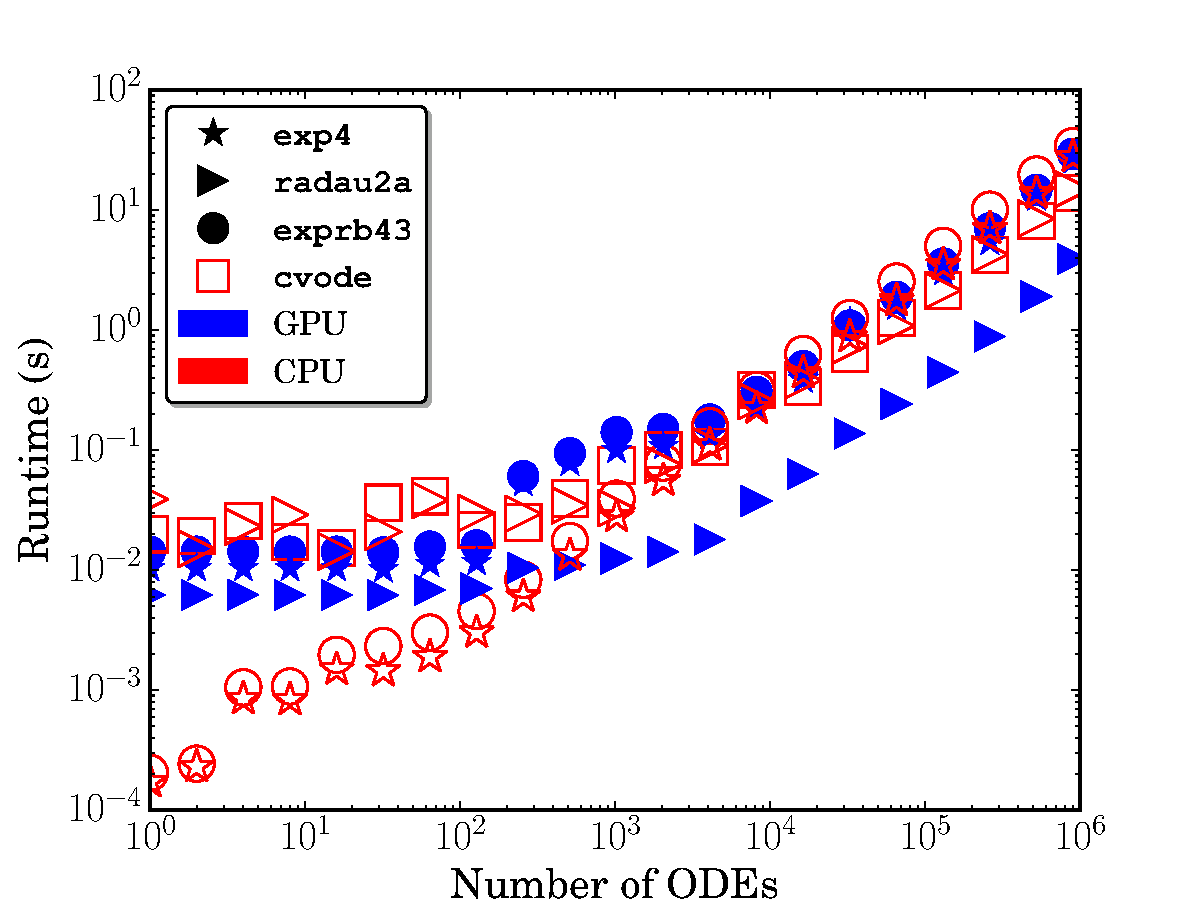
\includegraphics[width=\linewidth]{H2_1e-06_cpuvsgpu.pdf}
      \caption{$\delta t = \SI{1e-6}{\sec}$}   
  \end{subfigure}
  %\hfill
  \begin{subfigure}{0.49\textwidth}
      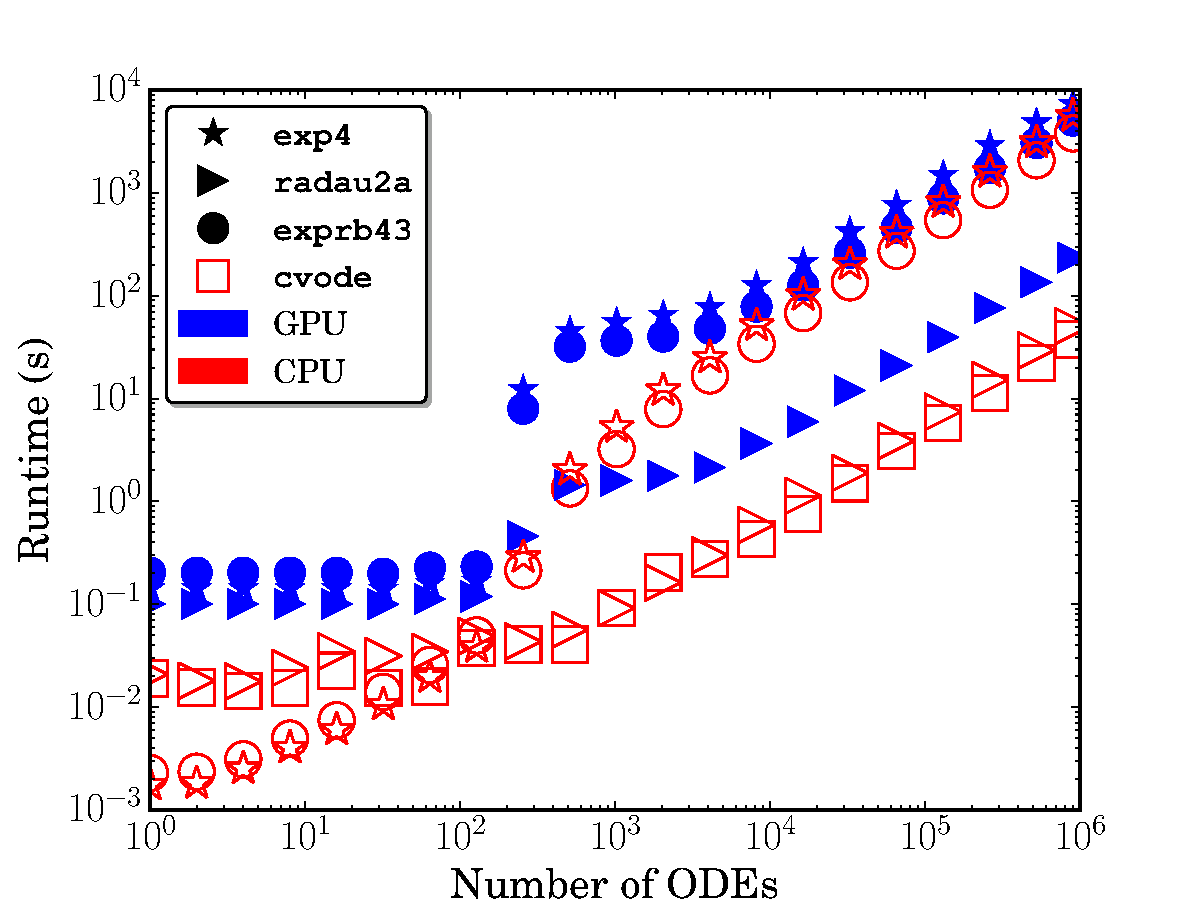
\includegraphics[width=\linewidth]{H2_1e-04_cpuvsgpu.pdf}
      \caption{$\delta t = \SI{1e-4}{\sec}$}
  \end{subfigure}
  \caption{Average runtimes of the integrators for the \ce{H2} mechanism at two different global timesteps. 
  CPU versions were run in parallel on six cores.}
  \label{F:H2_perf}
\end{figure}

Figure~\ref{F:H2_perf} shows the runtimes of the integrators for the \ce{H2} mechanism.
First, it is of note that the CPU \texttt{Radau-IIa} integrator is roughly equivalent with that of \texttt{CVODE} for the smaller global timestep, and only slightly slower \texttt{CVODE} for the larger timestep.
The GPU \texttt{Radau-IIa} integrator was at best $1.44\times$ slower than \texttt{CVODE}, and an average of $2.24\pm0.43\times$ slower for the smaller timestep (for more than 1024 ODEs, where the GPU becomes fully utilized).
For the larger timestep the performance decreased and was at best $3.17\times$ slower, and $8.25\pm2.98\times$ slower on average.
Both the CPU and GPU versions of the exponential integrators were significantly slower than the implicit integrators, although for the smaller timestep the GPU versions generally outperformed their CPU counterparts.
Although the \texttt{exprb43} and \texttt{exp4} integrators each only require three exponential matrix function approximations, \texttt{exprb43} is more expensive for a single step larger due to the extra chemical source term evaluations\slash matrix multiplications, and the higher-order phi function requirement.
As such, the CPU \texttt{exprb43} integrator generally is outperformed by the relatively more simple \texttt{exp4} integrator for the smaller timestep.
However, for the larger timestep with higher stiffness the expected order reduction~\cite{Bisetti:2012jw} of the \texttt{exp4} integrator makes it less efficient than \texttt{exprb43}.

\begin{figure}
  \centering
  \begin{subfigure}{0.49\textwidth}
      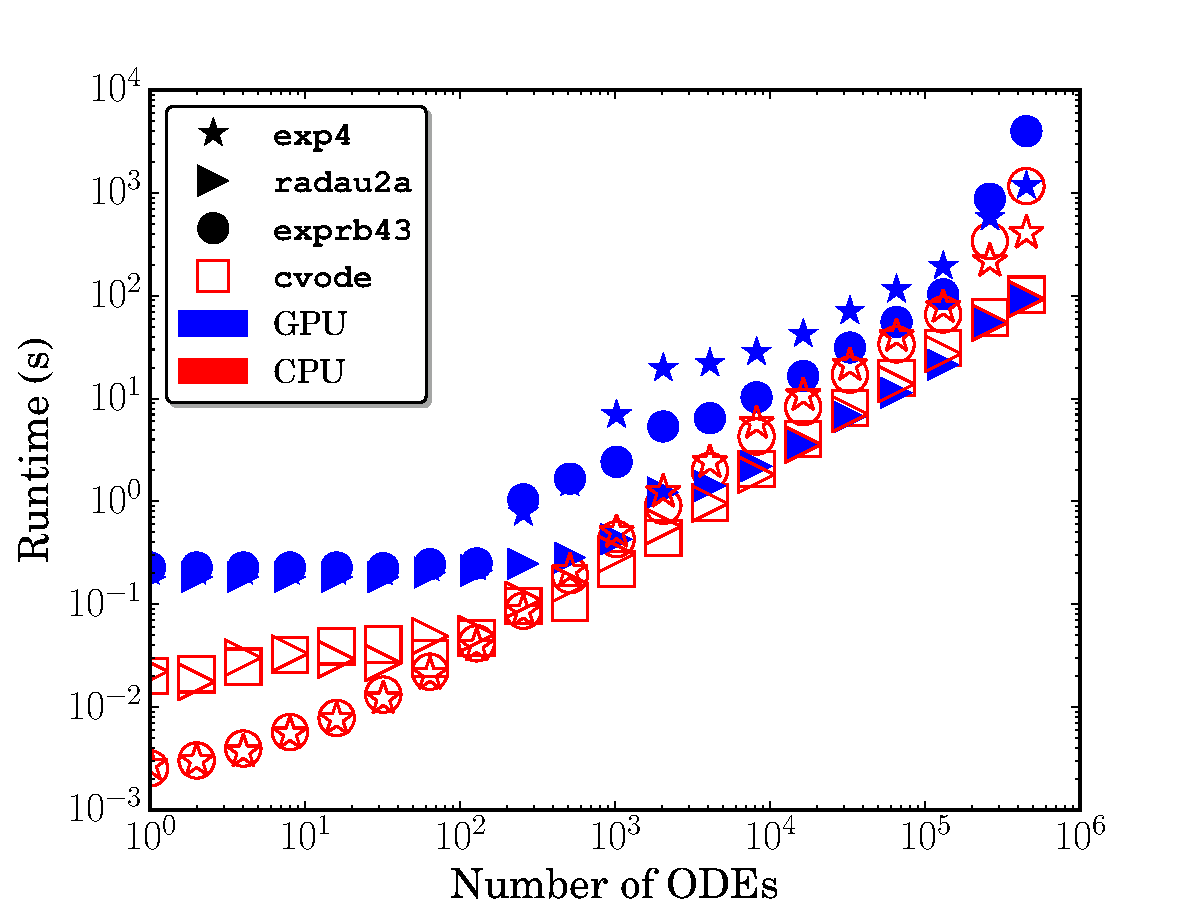
\includegraphics[width=\linewidth]{GRI_1e-06_cpuvsgpu.pdf}
      \caption{$\delta t = \SI{1e-6}{\sec}$}
  \end{subfigure}
  %\hfill
  \begin{subfigure}{0.49\textwidth}
      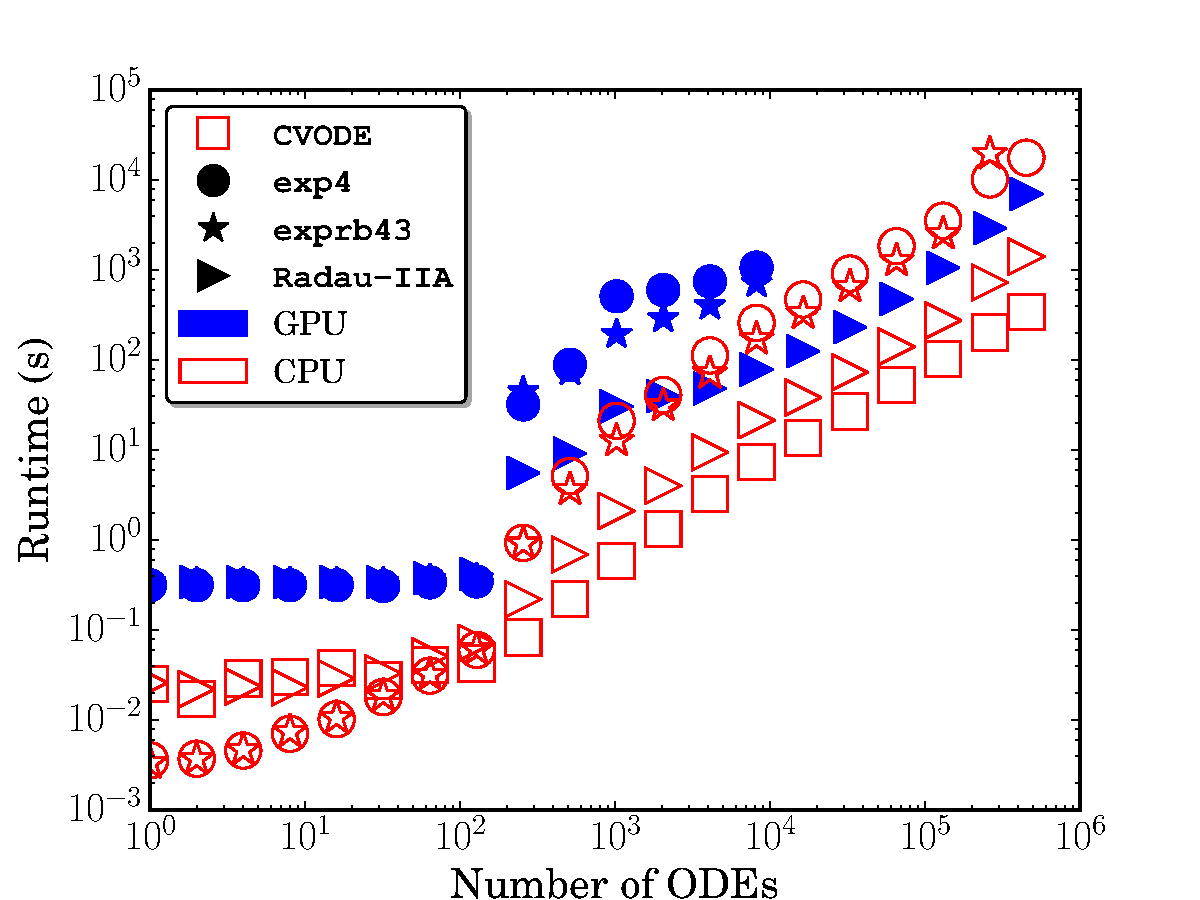
\includegraphics[width=\linewidth]{GRI_1e-04_cpuvsgpu.pdf}
      \caption{$\delta t = \SI{1e-4}{\sec}$}
  \end{subfigure}
  \caption{Average runtimes of the integrators for the GRI Mech.~3.0 mechanism at two different global timesteps. 
  CPU versions were run in parallel on six cores.
  Some of the longer running cases were omitted for clarity.}
  \label{F:GRI_perf}
\end{figure}

Figure~\ref{F:GRI_perf} shows the runtime of the integrators for the GRI mechanism.
Interestingly the GPU \texttt{Radau-IIa} integrator often outperforms the CPU version and \texttt{CVODE} for the smaller timestep; it is at best $1.46\times$ faster, and is on average $1.13\pm0.63\times$ slower.
For the larger timestep the performance of the GPU \texttt{Radau-IIa} integrator is again negatively impacted, dropping to a best case of $8.63\times$ slower, and $14.18\pm6.64\times$ slower on average.
For larger global timesteps, the range of required internal integrator timesteps is expected to increase~\cite{Niemeyer:2014aa}, and thus thread divergence will increase along with chemical stiffness for an ODE per-thread based integrator.
As the typical stiffness of the chemical ODE system increases when changing from the \ce{H2} mechanism to the GRI mechanism, this implies that thread divergence, rather than purely chemical stiffness, is the main performance limiter for the GPU \texttt{Radau-IIa} integrator.
Therefore, our future work will investigate strategies to reduce thread divergence, e.g., by adoption of an ODE per-block approach, or by re-ordering of ODEs to increase similarity of chemical stiffness inside a thread block.

Additionally two other trends of interest can be identified in Figure~\ref{F:GRI_perf}.
First, the larger global timestep is the only case studied where \texttt{CVODE} significantly outperforms the CPU \texttt{Radau-IIa} integrator.
This is likely due to the maturity of \texttt{CVODE} and years of optimization and tweaking.
Secondly, the performance of the CPU exponential integrators is similar to that of the implicit CPU integrators for the smaller timestep.
As the exponential integrators must only factorize a much smaller Hessenberg matrix, rather than that of the entire Jacobian as is required for the implicit integrators, the performance of the two integrator classes is roughly similar; thus the performance boost of the exponential integrators is expected to grow with mechanism size.
However, as the stiffness is increased, e.g., as in the large timestep case, the stability characteristics of the implicit integrators again makes them more favorable.
Thus the exponential integrators may be more efficient than the implicit integrators for moderately stiff systems (i.e., with small timesteps) of larger chemical mechanisms.

\subsection{Effect of Shared Memory Caching}
\label{S:smem}
The effectiveness of the shared memory caching scheme was evaluated in several cases by comparing the mean runtime of the integrators using rate and analytical Jacobian subroutines generated with and without the caching algorithm enabled.
A typical speedup of $\sim\SI{5}{\percent}$ was seen for the smaller global timestep cases, while a $\sim\SI{10}{\percent}$ speedup was observed for the larger timestep cases.
This difference is due to larger number of chemical source term and Jacobian evaluations required for the larger timestep cases.
In certain cases for the GRI mechanism, even larger speedups were observed, e.g. a \SI{24.4}{\percent} speedup with \texttt{exp4} for \SI{131072} ODEs and the \SI{1e-6}{\s} timestep, and a \SI{13.2}{\percent} speedup with \text{Radau-IIa} for \SI{32768} ODEs and the \SI{1e-4}{\s} timestep.


\subsection{Limitations of the one ODE per-thread approach}
During work on this paper, it was discovered that significant issues exist for the implementation of implicit and semi-implicit chemical-kinetic integrators on the GPU.
Namely, the size of the Jacobian itself places severe restrictions on either the maximum allowable mechanism size, or the total number of ODEs that can be solved concurrently.
For instance, the \texttt{Radau-IIA} solver requires storage of the Jacobian, as well as a LU factorized and a complex LU factorized matrix of the same size.
Similarly, the exponential integrators require storage of the Jacobian, the Hessenberg matrix and vector subspace resulting from the Arnoldi process and the corresponding exponential of the Hessenberg matrix.
While the Hessenberg matrix, exponential Hessenberg matrix, and vector subspaces can be smaller than the full Jacobian (e.g., by limiting the maximum Kyrlov subspace size), for the sake of simplicity in this analysis we shall assume they are full sized.
This implies that the storage requirements per ODE solved concurrently scales as $\mathcal{O}\left(3 \times N_s^2\right)$ for the \texttt{Radau-IIA} and at most $\mathcal{O}\left(4 \times N_s^2\right)$ for the exponential integrators, where $N_s$ is the number of species in the mechanism.

One method of storing these matrices (and other integrator variables) is in per-thread local memory.
This is advantageous from a programming standpoint, as it ensures coalesced memory access and simplifies indexing.
In CUDA however, all threads are limited to a maximum of \SI{512}{\kilo\byte} local memory, or \SI{64000} double precision floating point numbers.
This limits the maximum mechanism size to relatively small numbers, as seen in Table~\ref{T:size_limits}.

Additionally, the Jacobian and associated matricies can be pre-allocated in global memory, and thus the total global memory is split between all threads in a given kernel launch.
In this work, a Tesla C2075 GPU was used, and recent GPU-based chemical kinetic integration studies used similar models~\cite{Shi:2011aa,Niemeyer:2011aa,Shi:2012aa,Le2013596,Stone:2013aa,Niemeyer:2014aa}
Assuming a reasonable launch configuration of \SI{64} per block, with \SI{8} per streaming multiprocessor as on a C2050, we are limited to a maximum of $\sim$ \SI{419000000} threads (i.e. separate ODEs) per kernel launch.
For a \SI{6}{\giga\byte} global memory size, this works out to just \SI{178} available per thread.
Even assuming a more reasonable \SI{10000} threads, or low \SI{10000} threads per kernel launch, each thread is limited to just \SI{7500} and \SI{75000} doubles correspondingly.
The resulting (approximate) maximum mechanism sizes are listed in Table~\ref{T:size_limits}.

In this study, even the USC mechanism with only 111 species caused the GPU to run out of local thread memory for all three GPU integrators.
As one potential benefit of GPU based integration algorithms is to allow use of larger, say 100--200 species, skeletal mechanisms in general reacting flow by acceleration of chemical kinetic integration compared to CPU integrators, these restrictive mechanism size limits pose a large issue.
A chemical kinetic Jacobian based on species concentrations instead of species mass fractions exhibits significantly greater sparsity~\cite{Lu:2009gh}, and thus may relax the mechanism size limits imposed by Jacobian storage.
This is an avenue that will be explored in future work.

\begin{table}[tbp]
\centering
\begin{tabular}{@{}l l l l@{}}
 \toprule
& \multicolumn{3}{c}{Mechanism Size Limit} \\
Memory Type & \texttt{Radau-IIA} & \texttt{exp4} & \texttt{exprb43} \\
\midrule
Local	    & 146 & 126 & 126 \\

Global (max)	    & 7 & 6 & 6 \\
Global (reasonable) & 50 & 43 & 43 \\
Global (low) & 158 & 136 & 136 \\
\bottomrule
\end{tabular}
\caption{
Approximate mechanism size limits for the various GPU integrators based on per-thread local memory limits, and global memory limits.
``Max'', ``reasonable'', and ``low'' refer to kernel launches with a total of \SI{419000000}, \SI{100000} and \SI{10000} threads respectively
}
\label{T:size_limits}
\end{table}

%%%%%%%%%%%%%%%%%%%%%%%%%%%%%%%%%%%%%%%%%%%%
\section{Conclusions}
%%%%%%%%%%%%%%%%%%%%%%%%%%%%%%%%%%%%%%%%%%%%


%%%%%%%%%%%%%%%%%%%%%%%%%%%%%%%%%%%%%%%%%%%%%%%%%%%%%%%%%%%%%%%%%%%%%%
\section*{Acknowledgments}

This material is based upon work supported by the National Science Foundation under Grant Nos.~1534688 and 1535065.


\pagebreak

\bibliography{refs}
\bibliographystyle{elsarticle-num}

\end{document}
